\documentclass[
11pt, % The default document font size, options: 10pt, 11pt, 12pt
%codirector, % Uncomment to add a codirector to the title page
]{charter} 


% El títulos de la memoria, se usa en la carátula y se puede usar el cualquier lugar del documento con el comando \ttitle
\titulo{Detección de anomalías en servicio de TV-over-IP mediante autoencoder LSTM} 

% Nombre del posgrado, se usa en la carátula y se puede usar el cualquier lugar del documento con el comando \degreename
%\posgrado{Carrera de Especialización en Sistemas Embebidos} 
%\posgrado{Carrera de Especialización en Internet de las Cosas} 
\posgrado{Carrera de Especialización en Inteligencia Artificial}
%\posgrado{Maestría en Sistemas Embebidos} 
%\posgrado{Maestría en Internet de las cosas}

% Tu nombre, se puede usar el cualquier lugar del documento con el comando \authorname
% IMPORTANTE: no omitir titulaciones ni tildación en los nombres, también se recomienda escribir los nombres completos (tal cual los tienen en su documento)
\autor{Ing. Christopher Charaf}

% El nombre del director y co-director, se puede usar el cualquier lugar del documento con el comando \supname y \cosupname y \pertesupname y \pertecosupname
\director{Título y Nombre del director}
\pertenenciaDirector{buscando} 
\codirector{} % para que aparezca en la portada se debe descomentar la opción codirector en los parámetros de documentclass
\pertenenciaCoDirector{FIUBA}

% Nombre del cliente, quien va a aprobar los resultados del proyecto, se puede usar con el comando \clientename y \empclientename
\cliente{Kaltura Inc.}
\empresaCliente{Kaltura Inc.}
 
\fechaINICIO{24 de junio de 2025}		%Fecha de inicio de la cursada de GdP \fechaInicioName
\fechaFINALPlan{20 de Octubre de 2025} 	%Fecha de final de cursada de GdP
\fechaFINALTrabajo{15 de diciembre de 2025}	%Fecha de defensa pública del trabajo final


\begin{document}

\maketitle
\thispagestyle{empty}
\pagebreak


\thispagestyle{empty}
{\setlength{\parskip}{0pt}
\tableofcontents{}-
}
\pagebreak


\section*{Registros de cambios}
\label{sec:registro}


\begin{table}[ht]
\label{tab:registro}
\centering
\begin{tabularx}{\linewidth}{@{}|c|X|c|@{}}
\hline
\rowcolor[HTML]{C0C0C0} 
Revisión & \multicolumn{1}{c|}{\cellcolor[HTML]{C0C0C0}Detalles de los cambios realizados} & Fecha      \\ \hline
0      & Creación del documento                                 &\fechaInicioName \\ \hline
%1      & Se completa hasta el punto 5 inclusive                & {día} de {mes} de 202X \\ \hline
%2      & Se completa hasta el punto 9 inclusive
%		  Se puede agregar algo más \newline
%		  En distintas líneas \newline
%		  Así                                                    & {día} de {mes} de 202X \\ \hline
%3      & Se completa hasta el punto 12 inclusive                & {día} de {mes} de 202X \\ \hline
%4      & Se completa el plan	                                 & {día} de {mes} de 202X \\ \hline

% Si hay más correcciones pasada la versión 4 también se deben especificar acá

\end{tabularx}
\end{table}

\pagebreak



\section*{Acta de constitución del proyecto}
\label{sec:acta}

\begin{flushright}
Buenos Aires, \fechaInicioName
\end{flushright}

\vspace{2cm}

Por medio de la presente se acuerda con el \authorname\hspace{1px} que su Trabajo Final de la \degreename\hspace{1px} se titulará ``\ttitle'' y consistirá en \textbf{la implementación de un sistema de detección de anomalías en un servicio de TV-over-IP mediante un autoencoder LSTM}. El trabajo tendrá un presupuesto preliminar estimado de 600 horas y un costo estimado de \$ 7000, con fecha de inicio el \fechaInicioName\hspace{1px} y fecha de presentación pública el \fechaFinalName.

Se adjunta a esta acta la planificación inicial.

\vfill

% Esta parte se construye sola con la información que hayan cargado en el preámbulo del documento y no debe modificarla
\begin{table}[ht]
\centering
\begin{tabular}{ccc}
\begin{tabular}[c]{@{}c@{}}Dr. Ing. Ariel Lutenberg \\ Director posgrado FIUBA\end{tabular} & \hspace{2cm} & \begin{tabular}[c]{@{}c@{}}\clientename \\ \empclientename \end{tabular} \vspace{2.5cm} \\ 
\multicolumn{3}{c}{\begin{tabular}[c]{@{}c@{}} \supname \\ Director del Trabajo Final\end{tabular}} \vspace{2.5cm} \\
\end{tabular}
\end{table}




\section{1. Descripción técnica-conceptual del proyecto a realizar}
\label{sec:descripcion}

El presente proyecto tiene como objetivo desarrollar un sistema de detección de anomalías en tiempo real aplicado a un servicio de televisión por protocolo de Internet (TV-over-IP) basado en interfaces de programación de aplicaciones (API). Este servicio es monitoreado mediante métricas recolectadas a través de una herramienta de acumulacion de métricas llamada Prometheus, con una frecuencia de muestreo de 30 segundos. El sistema propuesto busca identificar comportamientos inusuales o fallos en el servicio mediante la reconstrucción de secuencias de métricas utilizando un modelo Autoencoder basado en redes neuronales de memoria a largo y corto plazo (LSTM, por sus siglas en inglés: \textit{Long Short-Term Memory}).

La empresa cliente dee este proyecto es "Kaltura Inc.", la cual provee servicios de TV-over-IP sobre infraestructura en la nube de Amazon Web Services (AWS). Esta empresa se enfrenta al desafío creciente de modernizar sus herramientas de monitoreo para mejorar la capacidad de reacción ante fallos en producción, sin depender exclusivamente de soluciones externas. Por este motivo, este desarrollo responde a una necesidad concreta del área de operaciones y calidad de servicio de la organización frente a sus clientes.

Actualmente, los métodos tradicionales de monitoreo utilizan umbrales fijos o alertas manuales, lo cual resulta ineficiente frente a comportamientos no triviales o patrones de uso dinámicos. Además, muchas herramientas de monitoreo de terceros requieren la exposición de métricas internas a servicios externos, por lo que compromete  la privacidad de los datos y aumenta la propensión a ataques. En contraste, este proyecto propone una solución propietaria, basada en aprendizaje automático, que permita detectar anomalías de manera autónoma, no invasiva y segura.

Desde el punto de vista técnico, el modelo recibirá como entrada ventanas deslizantes de tiempo compuestas por un número a definir de métricas técnicas que reflejan el rendimiento del servicio en tiempo real. Se utilizarán técnicas de ingeniería de características (\textit{feature engineering}) como la codificación cíclica del horario y variables contextuales que representen ventanas de mantenimiento y fines de semana para mejorar la sensibilidad del modelo frente a patrones estacionales.

Se empleará una arquitectura LSTM Autoencoder que aprende a reconstruir secuencias temporales multivariadas. Si el error de reconstrucción excede un umbral previamente definido, se considera que ocurrió una anomalía. En caso de detección, se emitirán alertas automáticas a través de la plataforma de alertas Opsgenie y se generarán enlaces a paneles de visualización de métricas como Grafana con el contexto temporal de la anomalía.

Esta propuesta se encuentra actualmente en su etapa inicial de planeamiento, donde se están definiendo tanto la arquitectura del modelo como las herramientas de integración con el ecosistema de monitoreo ya existente. La innovación principal reside en la aplicación de redes neuronales recurrentes para detección de anomalías directamente dentro del entorno técnico de la empresa, sin depender de soluciones comerciales de terceros. Esto refuerza la privacidad de los datos sensibles del sistema y de los usuarios, y permite una mayor adaptabilidad a los cambios en el comportamiento del servicio.

En comparación con el estado del arte, esta solución se destaca por su enfoque específico a servicios basados en API en tiempo real, su integración directa con herramientas de acumulación de métricas Prometheus y Grafana y por aplicar técnicas avanzadas de aprendizaje profundo en lugar de reglas estáticas. Esto la convierte en una alternativa más precisa, segura, escalable y personalizada que herramientas convencionales de detección de anomalías y alertas nativas de Grafana.

Cabe mencionar que no existen fuentes de financiamiento externo ni convenios públicos involucrados. El proyecto se desarrolla como parte del trabajo profesional del autor, y de acuerdo con el contrato vigente con la empresa, la propiedad intelectual de todos los entregables pertenece a la organización.

El cliente interno de este desarrollo es el área de operaciones de la empresa, que valora especialmente la capacidad de detección proactiva de incidentes, la integración fluida con su infraestructura existente y la reducción de falsos positivos. Necesita una solución confiable, sustentable y alineada con sus políticas de seguridad.

En la figura 1 se presenta el diagrama en bloques del sistema. Se observa que el flujo de datos comienza con la recolección de métricas desde Prometheus a través de su API, las cuales se almacenan en un marco de datos (\textit{dataframe}) y luego se someten a un proceso de preprocesamiento e ingeniería de características. A continuación, estas métricas son introducidas en un modelo Autoencoder basado en redes LSTM, compuesto por un codificador (\textit{encoder}) y un decodificador (\textit{decoder}), que tiene como objetivo reconstruir la secuencia original de datos. El sistema evalúa el error de reconstrucción de dichas métricas y lo compara contra un umbral definido: si el error excede dicho umbral, se considera que ocurrió una anomalía. En ese caso, se dispara una alerta automática hacia Opsgenie y se genera un enlace contextual hacia un panel de visualización en Grafana, lo que permite al equipo de operaciones inspeccionar el evento detectado con información visual en tiempo real. 

Si no se detecta anomalía, el sistema continúa procesando los siguientes datos de forma continua y en tiempo real. 

 

\begin{figure}[htpb]
\centering 
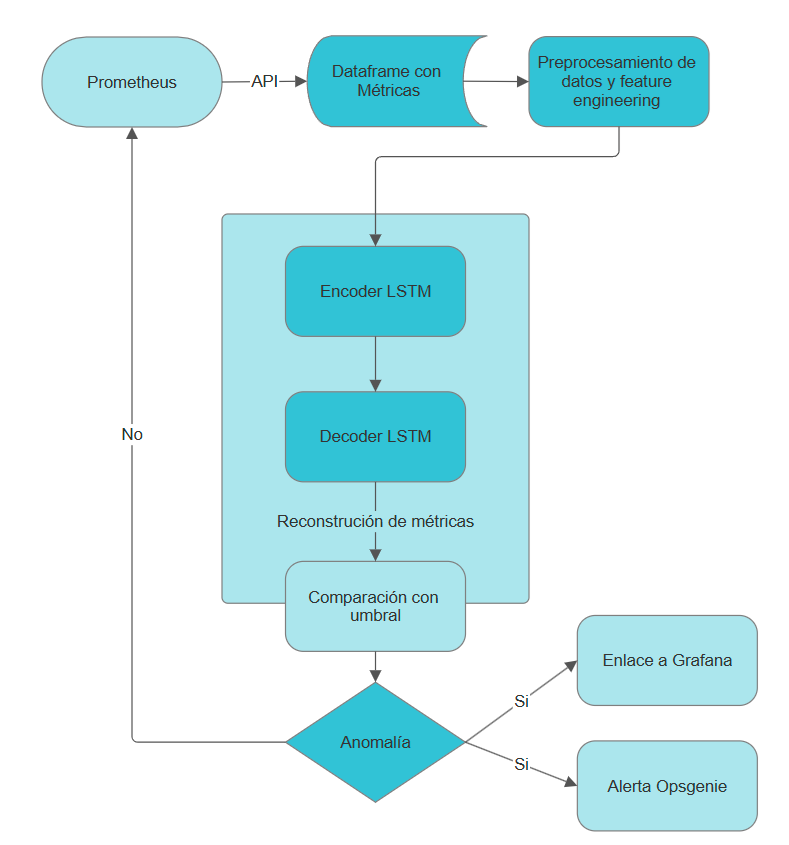
\includegraphics[width=.65\textwidth]{./Figuras/diag.png}
\caption{Diagrama en bloques del sistema.}
\label{fig:diagBloques}
\end{figure}

\vspace{25px}

\section{2. Identificación y análisis de los interesados}
\label{sec:interesados}
\begin{table}[ht]
%\caption{Identificación de los interesados}
%\label{tab:interesados}
\begin{tabularx}{\linewidth}{@{}|l|X|X|l|@{}}
\hline
\rowcolor[HTML]{C0C0C0} 
Rol           & Nombre y Apellido & Organización 	& Puesto 	\\ \hline
Auspiciante   &           \clientename        &  \clientename             	&      Departamento de soporte y operaciones 	\\ \hline
Responsable   & \authorname       & FIUBA        	& Alumno 	\\ \hline
Orientador    & \supname	      & \pertesupname 	& Director del Trabajo Final \\ \hline
Usuario final &       \clientename            &         \clientename     	&   Departamento de soporte y operaciones     	\\ \hline
\end{tabularx}
\end{table}


\begin{itemize}
	\item Orientador: a definir.
	\item Auspiciante: será el mismo usuario final de la solución, valora costos y organización en los procesos automatizados. 
\end{itemize}


\section{3. Propósito del proyecto}
\label{sec:proposito}
El propósito del proyecto es diseñar e implementar un sistema inteligente que permita detectar anomalías en tiempo real dentro de un servicio de televisión por protocolo de \textit{Internet} (\textit{TV-over-IP}), basado en APIs y desplegado sobre infraestructura en la nube. Mediante el uso de un modelo \textit{autoencoder} basado en redes neuronales LSTM, se busca brindar a la empresa una herramienta robusta y segura para el monitoreo continuo de métricas técnicas clave; esta solución mejora su capacidad de respuesta ante incidentes, minimiza el tiempo de inactividad del servicio y garantiza una mayor calidad de experiencia para sus usuarios finales. 

\section{4. Alcance del proyecto}
\label{sec:alcance}

El proyecto \textbf{incluye}:
\begin{itemize}
    \item La definición y análisis de métricas críticas del servicio de TV-over-IP recolectadas desde Prometheus mediante su API.
    \item El diseño e implementación de una serie de procesos(\textit{pipeline}) de procesamiento de datos, incluyendo:
    \begin{itemize}
        \item Normalización de variables.
        \item \textit{Feature engineering} (codificación cíclica de hora, día, etc.).
        \item Construcción de ventanas deslizantes para series temporales.
    \end{itemize}
    \item El desarrollo de un modelo de detección de anomalías basado en Autoencoder LSTM, entrenado para reconstruir secuencias multivariadas normales.
    \item La integración del sistema con herramientas de monitoreo existentes:
    \begin{itemize}
        \item Generación de alertas automáticas vía Opsgenie.
        \item Enlace contextual a paneles de Grafana.
    \end{itemize}
    \item La validación del sistema en un entorno de producción con datos reales históricos.
    \item La elaboración de documentación técnica y funcional del prototipo.
\end{itemize}
El presente proyecto \textbf{no incluye}:

\begin{itemize}
    \item El desarrollo de interfaces gráficas adicionales fuera de Grafana.
    \item La implementación de acciones correctivas automáticas posteriores a la detección de anomalías.
    \item La gestión directa de recursos en AWS ni tareas de infraestructura subyacente (como escalado automático, balanceo de carga, etc.).
\end{itemize}



\section{5. Supuestos del proyecto}
\label{sec:supuestos}

Para el desarrollo del presente proyecto se supone que:

\begin{enumerate}
    \item \clientename  \space brindará acceso a las métricas necesarias a través de su instancia de Prometheus mediante API REST, así como también a sus paneles de visualización en Grafana.
    \item El \textit{dataframe} histórico utilizado para entrenamiento estará disponible, completo y será representativo del comportamiento normal del sistema en condiciones reales de operación.
    \item Se contará con los recursos computacionales necesarios (por ejemplo, GPU opcional) para el entrenamiento del modelo LSTM Autoencoder en un entorno controlado por \clientename.
    \item Las herramientas de integración como Opsgenie y Grafana ya están operativas y disponibles para pruebas dentro de la infraestructura de la empresa.
    \item No se producirán cambios drásticos en el comportamiento del servicio durante el período de entrenamiento y validación que comprometan la utilidad del modelo.
    \item El equipo de operaciones colaborará en la validación funcional del sistema, especialmente en la evaluación de falsos positivos y en el ajuste del umbral de alerta en base a estándares existentes en la empresa.
    \item Las condiciones legales, de seguridad y de confidencialidad establecidas en el contrato del autor con la empresa se mantendrán vigentes y permitirán el desarrollo del proyecto sin restricciones externas.
\end{enumerate}


\section{6. Requerimientos}
\label{sec:requerimientos}


\begin{enumerate}
    \item \textbf{Requerimientos funcionales}:
 1.1. El sistema debe ser capaz de recolectar métricas técnicas desde Prometheus a través de su API REST. (\textbf{Alta prioridad})

 1.2. El sistema debe construir ventanas deslizantes de 20 pasos temporales (10 minutos) con una frecuencia de muestreo de 30 segundos. (\textbf{Alta prioridad})

 1.3. El sistema debe aplicar técnicas de normalización y codificación cíclica de variables temporales como \verb|hour_sin| y \verb|hour_cos|. (\textbf{Alta prioridad})

 1.4. El modelo debe reconstruir secuencias multivariadas. (\textbf{Alta prioridad})

 1.5. El sistema debe detectar anomalías cuando el error de reconstrucción supere un umbral configurable. (\textbf{Alta prioridad})

 1.6. En caso de anomalía, el sistema debe enviar una alerta automática a través de Opsgenie. (\textbf{Media prioridad})

 1.7. El sistema debe incluir un enlace a Grafana que muestre el contexto temporal de la anomalía detectada. (\textbf{Media prioridad})
    \item \textbf{Requerimientos de documentación}:

 2.1. Se debe entregar documentación técnica del modelo, su entrenamiento, configuración y uso. (\textbf{Alta prioridad})

 2.2. Se debe entregar una memoria del trabajo final con descripción funcional, arquitectura y resultados. (\textbf{Alta prioridad})

 2.3. Se debe incluir una guía básica de despliegue e integración del sistema en entornos compatibles. (\textbf{Media prioridad})
    \item \textbf{Requerimientos de \textit{testing} y validación}:

 3.1. El sistema debe ser validado sobre datos históricos que representen el comportamiento normal del sistema. (\textbf{Alta prioridad})

 3.2. Se deben generar métricas de desempeño como tasa de falsos positivos y precisión de detección. (\textbf{Alta prioridad})

 3.3. El umbral de error debe ser calibrado en conjunto con el equipo de operaciones. (\textbf{Media prioridad})
    \item \textbf{Requerimientos de interfaz}:

 4.1. El sistema no debe contar con una interfaz gráfica propia, pero debe integrarse con visualizaciones (\textit{dashboards}) existentes en Grafana. (\textbf{Alta prioridad})

 4.2. El mensaje de alerta debe incluir timestamp, métricas anómalas, y visualización de valores reales vs reconstruidos. (\textbf{Media prioridad})
    \item \textbf{Requerimientos de interoperatividad e integración}:

 5.1. El sistema debe integrarse con la instancia de Prometheus de la empresa. (\textbf{Alta prioridad})

 5.2. El sistema debe ser compatible con Grafana para visualización. (\textbf{Alta prioridad})

 5.3. El sistema debe ser capaz de emitir alertas en el formato requerido por Opsgenie. (\textbf{Media prioridad})
    \item \textbf{Requerimientos normativos y de seguridad}:

 6.1. El sistema no debe enviar datos a servicios externos no autorizados. (\textbf{Alta prioridad})

 6.2. Todo el procesamiento debe realizarse dentro de la red interna de la empresa o su infraestructura autorizada en AWS. (\textbf{Alta prioridad})

 6.3. El sistema debe respetar las políticas internas de privacidad y seguridad de la información establecidas por la empresa. (\textbf{Alta prioridad})
    \item \textbf{Requerimientos opcionales}:

 7.1. Incluir variables adicionales como \verb|weekday|, \verb|is_weekend|, \verb|is_night| en el \textit{feature engineering}. (\textbf{Opcional})

 7.2. Permitir ajuste dinámico del umbral de detección desde una configuración externa. (\textbf{Opcional}) 
\end{enumerate}
   
    
\section{7. Historias de usuarios (\textit{Product backlog})}
\label{sec:backlog}

Los \textbf{story points} se asignaron considerando tres factores:

\begin{itemize}
    \item \textbf{Complejidad técnica} (1 a 5)
    \item \textbf{Dificultad de implementación} (1 a 5)
    \item \textbf{Grado de incertidumbre} (1 a 5)

 Fórmula: \textbf{SP = Complejidad + Dificultad + Incertidumbre}
\end{itemize}

\begin{enumerate}
    \item \textbf{“Como ingeniero de monitoreo quiero recibir alertas automáticas cuando se detecten anomalías para poder reaccionar rápidamente y minimizar el impacto en el servicio.”}

 \textbf{Story points:} 8 (Complejidad: 3, Dificultad: 2, Incertidumbre: 3)
    \item \textbf{“Como desarrollador de datos quiero procesar las métricas recolectadas y convertirlas en secuencias temporales con variables adicionales para entrenar el modelo.”}

 \textbf{Story points:} 7 (Complejidad: 3, Dificultad: 2, Incertidumbre: 2)
    \item \textbf{“Como operador del sistema quiero que cada alerta contenga un enlace directo a un panel de Grafana para visualizar rápidamente la anomalía detectada.”}

 \textbf{Story points:} 5 (Complejidad: 2, Dificultad: 1, Incertidumbre: 2)
    \item \textbf{“Como responsable de infraestructura quiero que el sistema funcione dentro de nuestra red privada para evitar exponer datos sensibles a servicios externos.”}

 \textbf{Story points:} 6 (Complejidad: 2, Dificultad: 2, Incertidumbre: 2)
    \item \textbf{“Como científico de datos quiero entrenar el modelo sobre datos históricos para que aprenda el comportamiento normal del sistema.”}

 \textbf{Story points:} 6 (Complejidad: 2, Dificultad: 2, Incertidumbre: 2)
    \item \textbf{“Como técnico de soporte quiero acceder a un log con las métricas reales y reconstruidas al momento de la anomalía para facilitar el diagnóstico del incidente.”}

 \textbf{Story points:} 5 (Complejidad: 2, Dificultad: 2, Incertidumbre: 1)
\end{enumerate}


\section{8. Entregables principales del proyecto}
\label{sec:entregables}

\begin{itemize}
    \item \textbf{Documentación técnica del sistema}:

 Contendrá la descripción de la arquitectura del modelo, el flujo de procesamiento de datos, los componentes implementados y las herramientas utilizadas (Prometheus, Grafana, Opsgenie, entre otras).
    \item \textbf{Memoria del trabajo final}:

 Documento completo que incluye la descripción técnica-conceptual, estado del arte, objetivos, metodología, implementación, resultados obtenidos y conclusiones.
    \item \textbf{Código fuente del sistema}:

 Scripts y módulos desarrollados para el procesamiento de datos, entrenamiento del modelo, inferencia y generación de alertas. El código será entregado con instrucciones de ejecución y dependencias requeridas.
    \item \textbf{Modelo LSTM Autoencoder entrenado}:

 Archivo con los pesos y la estructura del modelo entrenado, listo para su despliegue en entorno de validación o producción.
    \item \textbf{Pipeline de procesamiento de datos}:

 Conjunto de scripts que automatizan las etapas de recolección, transformación, normalización y estructuración de datos históricos en secuencias para el modelo.
    \item \textbf{Configuración de integración con Opsgenie y Grafana}:

 Archivos de configuración, ejemplos y plantillas para la conexión del sistema con los mecanismos de alerta y visualización en tiempo real utilizados por la empresa.
\end{itemize}
    

\section{9. Desglose del trabajo en tareas}
\label{sec:wbs}

\begin{enumerate}
\item Análisis y definición del sistema (40 h)
\begin{enumerate}
\item Revisión del estado del arte y casos similares (8 h)
\item Análisis de métricas disponibles en Prometheus (12 h)
\item Definición de requerimientos funcionales y no funcionales (10 h)
\item Diseño preliminar del sistema y definición del pipeline (10 h)
\end{enumerate}

\item Desarrollo del pipeline de datos (50 h)
\begin{enumerate}
\item Implementación del recolector de métricas desde Prometheus (10 h)
\item Desarrollo de preprocesamiento y normalización (12 h)
\item Implementación de ingeniería de variables temporales (10 h)
\item Construcción de ventanas deslizantes para series temporales (10 h)
\item Validación del pipeline con datos históricos (8 h)
\end{enumerate}

\item Desarrollo y entrenamiento del modelo (60 h)
\begin{enumerate}
\item Definición de arquitectura LSTM Autoencoder (10 h)
\item Implementación del modelo en Keras/TensorFlow (12 h)
\item Preparación del conjunto de entrenamiento y validación (10 h)
\item Entrenamiento del modelo con tuning de hiperparámetros (16 h)
\item Evaluación del desempeño con métricas objetivas (12 h)
\end{enumerate}

\item Integración con sistema de monitoreo (Grafana y Opsgenie) (35 h)
\begin{enumerate}
\item Diseño del mecanismo de alerta con umbral configurable (10 h)
\item Integración con Opsgenie para envío de alertas (8 h)
\item Generación de enlaces hacia dashboards de Grafana (7 h)
\item Pruebas de integración en entorno controlado (10 h)
\end{enumerate}

\item Validación, documentación y entregables (40 h)
\begin{enumerate}
\item Validación funcional con el equipo de operaciones (10 h)
\item Elaboración del informe de resultados y validación (8 h)
\item Redacción de la memoria técnica del proyecto (12 h)
\item Preparación de documentación de uso e integración (10 h)
\end{enumerate}
\end{enumerate}

\textbf{Cantidad total de horas: 225 h.}

\section{10. Diagrama de Activity On Node}
\label{sec:AoN}

\begin{table}[H]
\centering
\begin{tabular}{|>{\centering\arraybackslash}p{0.15\linewidth}|>{\raggedright\arraybackslash}p{0.33\linewidth}|>{\raggedright\arraybackslash}p{0.5\linewidth}|}
\hline
\rowcolor[HTML]{EFEFEF}
\textbf{Color} & \textbf{Grupo de tareas} & \textbf{Descripción} \\ \hline

\cellcolor[HTML]{FFF2CC} Amarillo claro & Grupo 1: Análisis y definición del sistema & Tareas relacionadas con el estudio preliminar, análisis de métricas, requisitos y diseño inicial. \\ \hline

\cellcolor[HTML]{DAE8FC} Celeste claro & Grupo 2: Desarrollo del pipeline de datos & Implementación del recolector de métricas, preprocesamiento, normalización y ventanas deslizantes. \\ \hline

\cellcolor[HTML]{E1D5E7} Violeta claro & Grupo 3: Desarrollo y entrenamiento del modelo & Definición de la arquitectura, implementación y evaluación del modelo LSTM Autoencoder. \\ \hline

\cellcolor[HTML]{F8CECC} Rosado claro & Grupo 4: Integración con sistema de monitoreo & Tareas de conexión con Opsgenie, configuración de alertas y enlaces hacia dashboards de Grafana. \\ \hline

\cellcolor[HTML]{D5E8D4} Verde claro & Grupo 5: Validación, documentación y entregables & Actividades de verificación, redacción del informe técnico y documentación final del proyecto. \\ \hline

\cellcolor[HTML]{FFFFFF} Blanco & Inicio / Fin & Representa los nodos de comienzo y cierre del proyecto. \\ \hline

\end{tabular}
\caption{Cuadro indicativo de colores del Diagrama AoN}
\end{table}


\begin{figure}[htpb]
\centering 
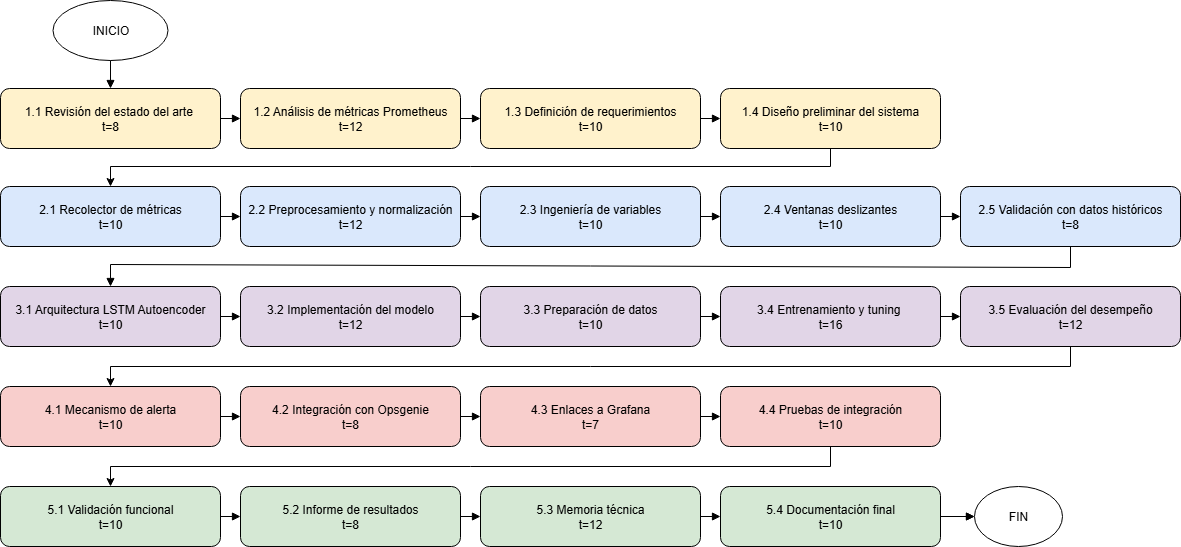
\includegraphics[width=1\textwidth]{./Figuras/AoN.png}
\caption{Diagrama de \textit{Activity on Node}.}
\label{fig:AoN}
\end{figure}



\section{11. Diagrama de Gantt}
\label{sec:gantt}
A continuación se presenta el diagrama de Gantt correspondiente al cronograma del proyecto. El mismo se muestra en formato apaisado con el objetivo de facilitar su lectura y visualización, permitiendo apreciar con claridad la secuencia temporal de las actividades planificadas, su duración estimada y su relación con el resto de las tareas. Este diagrama fue elaborado en base al desglose de tareas definido en el WBS (punto 9) y refleja la distribución efectiva del trabajo a lo largo del tiempo, considerando una carga de 3 horas diarias, días no laborables y períodos de vacaciones. 
\begin{landscape}
\begin{figure}[H]
\centering
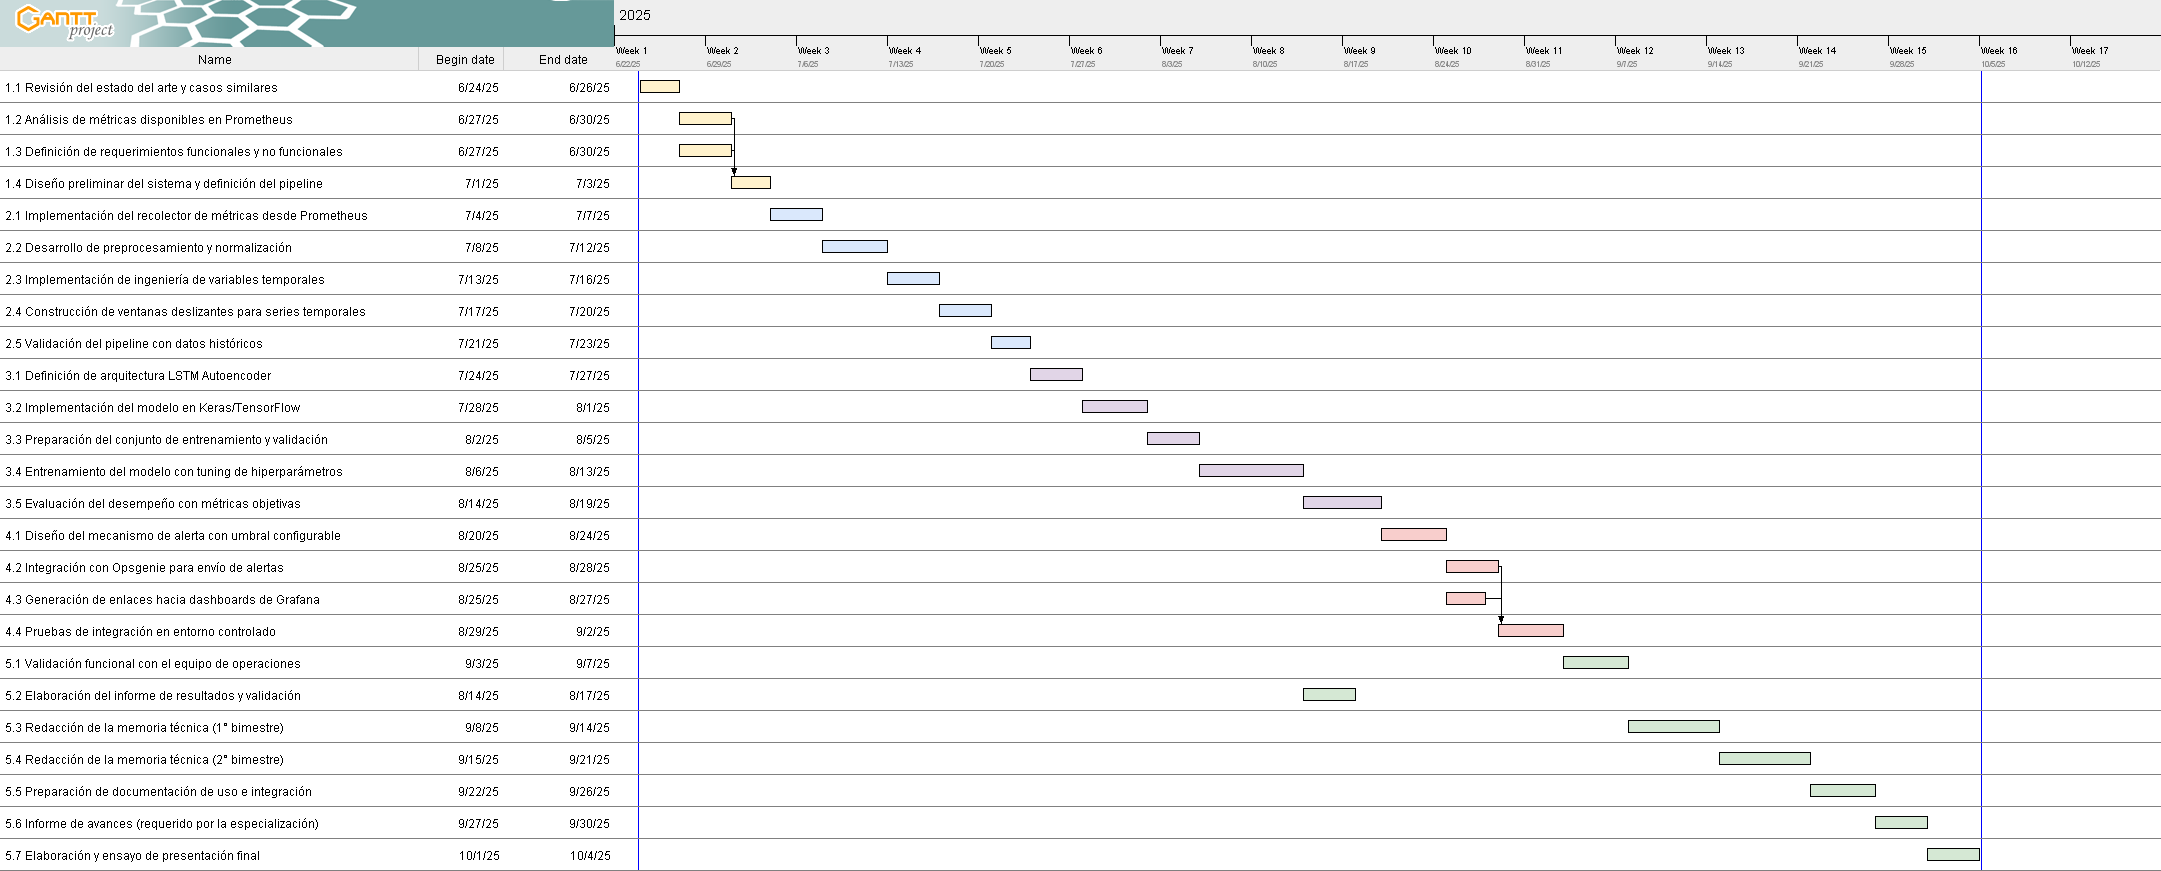
\includegraphics[width=\linewidth,keepaspectratio]{./Figuras/Gantt-2.png}
\caption{Diagrama de Gantt (apaisado).}
\label{fig:diagGantt}

\end{figure}
\end{landscape}



\section{12. Presupuesto detallado del proyecto}
\label{sec:presupuesto}

\begin{table}[H]
\centering
\begin{tabular}{|>{\raggedright\arraybackslash}p{0.5\linewidth}|>{\centering\arraybackslash}p{0.1\linewidth}|>{\centering\arraybackslash}p{0.2\linewidth}|>{\centering\arraybackslash}p{0.2\linewidth}|}
\hline
\textbf{Descripción} & \textbf{Cantidad (h)} & \textbf{Valor unitario (ARS)} & \textbf{Valor total (ARS)} \\
\hline
Análisis y definición del sistema & 40 & 6.000 & 240.000 \\\hline
Desarrollo del pipeline de datos & 50 & 6.000 & 300.000 \\\hline
Desarrollo y entrenamiento del modelo & 60 & 6.000 & 360.000 \\\hline
Integración con herramientas de monitoreo & 35 & 6.000 & 210.000 \\\hline
Validación, documentación y entregables & 40 & 6.000 & 240.000 \\
\hline
\textbf{Subtotal costos directos} & \textbf{225} &  & \textbf{1.350.000} \\
\hline
\end{tabular}
\caption{Presupuesto de costos directos del proyecto}
\end{table}
\begin{table}[H]
\centering
\begin{tabular}{|>{\raggedright\arraybackslash}p{0.25\linewidth}|>{\centering\arraybackslash}p{0.25\linewidth}|>{\centering\arraybackslash}p{0.25\linewidth}|>{\centering\arraybackslash}p{0.25\linewidth}|}
\hline
\textbf{Descripción} & \textbf{Cantidad} & \textbf{Valor unitario (ARS)} & \textbf{Valor total (ARS)} \\
\hline
Electricidad y conectividad (mensual estimado) & 3 meses & 15.000 & 45.000 \\\hline
Licencias de software y servicios en la nube(AWS)& 1 uso & 25.000 & 25.000 \\
\hline
\textbf{Subtotal costos indirectos} &  &  & \textbf{70.000} \\
\hline
\end{tabular}
\caption{Presupuesto de costos indirectos del proyecto}
\end{table}
\begin{center}
\textbf{Costo total del proyecto: \textcurrency~1.420.000 ARS}
\end{center}




\section{13. Gestión de riesgos}
\label{sec:riesgos}

\begin{consigna}{red}
a) Identificación de los riesgos (al menos cinco) y estimación de sus consecuencias:
 
Riesgo 1: detallar el riesgo (riesgo es algo que si ocurre altera los planes previstos de forma negativa)
\begin{itemize}
	\item Severidad (S): mientras más severo, más alto es el número (usar números del 1 al 10).\\
	Justificar el motivo por el cual se asigna determinado número de severidad (S).
	\item Probabilidad de ocurrencia (O): mientras más probable, más alto es el número (usar del 1 al 10).\\
	Justificar el motivo por el cual se asigna determinado número de (O). 
\end{itemize}   

Riesgo 2:
\begin{itemize}
	\item Severidad (S): X.\\
	Justificación...
	\item Ocurrencia (O): Y.\\
	Justificación...
\end{itemize}

Riesgo 3:
\begin{itemize}
	\item Severidad (S):  X.\\
	Justificación...
	\item Ocurrencia (O): Y.\\
	Justificación...
\end{itemize}


b) Tabla de gestión de riesgos:      (El RPN se calcula como RPN=SxO)

\begin{table}[htpb]
\centering
\begin{tabularx}{\linewidth}{@{}|X|c|c|c|c|c|c|@{}}
\hline
\rowcolor[HTML]{C0C0C0} 
Riesgo & S & O & RPN & S* & O* & RPN* \\ \hline
       &   &   &     &    &    &      \\ \hline
       &   &   &     &    &    &      \\ \hline
       &   &   &     &    &    &      \\ \hline
       &   &   &     &    &    &      \\ \hline
       &   &   &     &    &    &      \\ \hline
\end{tabularx}%
\end{table}

Criterio adoptado: 

Se tomarán medidas de mitigación en los riesgos cuyos números de RPN sean mayores a...

Nota: los valores marcados con (*) en la tabla corresponden luego de haber aplicado la mitigación.

c) Plan de mitigación de los riesgos que originalmente excedían el RPN máximo establecido:
 
Riesgo 1: plan de mitigación (si por el RPN fuera necesario elaborar un plan de mitigación).
  Nueva asignación de S y O, con su respectiva justificación:
  \begin{itemize}
	\item Severidad (S*): mientras más severo, más alto es el número (usar números del 1 al 10).
          Justificar el motivo por el cual se asigna determinado número de severidad (S).
	\item Probabilidad de ocurrencia (O*): mientras más probable, más alto es el número (usar del 1 al 10).
          Justificar el motivo por el cual se asigna determinado número de (O).
	\end{itemize}

Riesgo 2: plan de mitigación (si por el RPN fuera necesario elaborar un plan de mitigación).
 
Riesgo 3: plan de mitigación (si por el RPN fuera necesario elaborar un plan de mitigación).

\end{consigna}


\section{14. Gestión de la calidad}
\label{sec:calidad}

\begin{consigna}{red}
Elija al menos diez requerimientos que a su criterio sean los más importantes/críticos/que aportan más valor y para cada uno de ellos indique las acciones de verificación y validación que permitan asegurar su cumplimiento.

\begin{itemize} 
\item Req \#1: copiar acá el requerimiento con su correspondiente número.

\begin{itemize}
	\item Verificación para confirmar si se cumplió con lo requerido antes de mostrar el sistema al cliente. Detallar.
	\item Validación con el cliente para confirmar que está de acuerdo en que se cumplió con lo requerido. Detallar. 
\end{itemize}

\end{itemize}

Tener en cuenta que en este contexto se pueden mencionar simulaciones, cálculos, revisión de hojas de datos, consulta con expertos, mediciones, etc.  

Las acciones de verificación suelen considerar al entregable como ``caja blanca'', es decir se conoce en profundidad su funcionamiento interno.  

En cambio, las acciones de validación suelen considerar al entregable como ``caja negra'', es decir, que no se conocen los detalles de su funcionamiento interno.

\end{consigna}

\section{15. Procesos de cierre}    
\label{sec:cierre}

\begin{consigna}{red}
Establecer las pautas de trabajo para realizar una reunión final de evaluación del proyecto, tal que contemple las siguientes actividades:

\begin{itemize}
	\item Pautas de trabajo que se seguirán para analizar si se respetó el Plan de Proyecto original:\\
	 - Indicar quién se ocupará de hacer esto y cuál será el procedimiento a aplicar. 
	\item Identificación de las técnicas y procedimientos útiles e inútiles que se emplearon, los problemas que surgieron y cómo se solucionaron:\\
	 - Indicar quién se ocupará de hacer esto y cuál será el procedimiento para dejar registro.
	\item Indicar quién organizará el acto de agradecimiento a todos los interesados, y en especial al equipo de trabajo y colaboradores:\\
	  - Indicar esto y quién financiará los gastos correspondientes.
\end{itemize}

\end{consigna}

\end{document}